%%%%%%%%%%%%%%%%%%%% author.tex %%%%%%%%%%%%%%%%%%%%%%%%%%%%%%%%%%%
%
% template for chapters to the Handbook of Exoplanets
% modified by H. Deeg from the 'template.tex' provided by Springer for the svmult.cls class
% 20Mar 2016
%
%%%%%%%%%%%%%%%% Springer %%%%%%%%%%%%%%%%%%%%%%%%%%%%%%%%%%


% RECOMMENDED %%%%%%%%%%%%%%%%%%%%%%%%%%%%%%%%%%%%%%%%%%%%%%%%%%%
\documentclass[graybox,natbib,nosecnum]{svmult}
\bibpunct{(}{)}{;}{a}{}{,} % suppress commas between author-names and year

\pdfoutput=1   %forces use of pdflatex. Disable if you prefer to use .eps or .ps figures.
% choose options for [] as required from the list
% in the Reference Guide

\usepackage{mathptmx}       % selects Times Roman as basic font
\usepackage{helvet}         % selects Helvetica as sans-serif font
\usepackage{courier}        % selects Courier as typewriter font
\usepackage{type1cm}        % activate if the above 3 fonts are
                            % not available on your system

\usepackage{makeidx}         % allows index generation
\usepackage{graphicx}        % standard LaTeX graphics tool
\usepackage{units}        %
\usepackage{amssymb}        %
                             % when including figure files
\usepackage{multicol}        % used for the two-column index
\usepackage[bottom]{footmisc}% places footnotes at page bottom
\usepackage[normalem]{ulem}	% for strike-through of text with \sout{}  
\usepackage{hyperref}  %for hyperlinks


\usepackage{soul}   % for high-lighting of text
% see the list of further useful packages
% in the Reference Guide

% expansions of  journal abbreviations from bibtex entries by ADS
% adapted to Springer Basic style (no periods in abbreviations)
\newcommand*\aap{A\&A}
\let\astap=\aap
\newcommand*\aapr{A\&A Rev}
\newcommand*\aaps{A\&AS}
\newcommand*\actaa{Acta Astron}
\newcommand*\aj{AJ}
\newcommand*\ao{Appl Opt}
\let\applopt\ao
\newcommand*\apj{ApJ}
\newcommand*\apjl{ApJ}
\let\apjlett\apjl
\newcommand*\apjs{ApJS}
\let\apjsupp\apjs
\newcommand*\aplett{Astrophys Lett}
\newcommand*\apspr{Astrophys Space Phys Res}
\newcommand*\apss{Ap\&SS}
\newcommand*\araa{ARA\&A}
\newcommand*\azh{AZh}
\newcommand*\baas{BAAS}
\newcommand*\bac{Bull astr Inst Czechosl}
\newcommand*\bain{Bull Astron Inst Netherlands}
\newcommand*\caa{Chinese Astron Astrophys}
\newcommand*\cjaa{Chinese J Astron Astrophys}
\newcommand*\fcp{Fund Cosmic Phys}
\newcommand*\gca{Geochim Cosmochim Acta}
\newcommand*\grl{Geophys Res Lett}
\newcommand*\iaucirc{IAU Circ}
\newcommand*\icarus{Icarus}
\newcommand*\jcap{J Cosmology Astropart Phys}
\newcommand*\jcp{J Chem Phys}
\newcommand*\jgr{J Geophys Res}
\newcommand*\jqsrt{J Quant Spectr Rad Transf}
\newcommand*\jrasc{JRASC}
\newcommand*\memras{MmRAS}
\newcommand*\memsai{Mem Soc Astron Italiana}
\newcommand*\mnras{MNRAS}
\newcommand*\na{New A}
\newcommand*\nar{New A Rev}
\newcommand*\nat{Nature}
\newcommand*\nphysa{Nucl Phys A}
\newcommand*\pasa{PASA}
\newcommand*\pasj{PASJ}
\newcommand*\pasp{PASP}
\newcommand*\physrep{Phys Rep}
\newcommand*\physscr{Phys Scr}
\newcommand*\planss{Planet Space Sci}
\newcommand*\pra{Phys Rev A}
\newcommand*\prb{Phys Rev B}
\newcommand*\prc{Phys Rev C}
\newcommand*\prd{Phys Rev D}
\newcommand*\pre{Phys Rev E}
\newcommand*\prl{Phys Rev Lett}
\newcommand*\procspie{Proc SPIE}
\newcommand*\qjras{QJRAS}
\newcommand*\rmxaa{Rev Mexicana Astron Astrofis}
\newcommand*\skytel{S\&T}
\newcommand*\solphys{Sol Phys}
\newcommand*\sovast{Soviet Ast}
\newcommand*\ssr{Space Sci Rev}
\newcommand*\zap{ZAp}


\newcommand{\hbindex}[1]{\hl{#1}\index{#1}}  %highlights index entries

\makeindex             % used for the subject index
                       % please use the style svind.ist with
                       % your makeindex program

%%%%%%%%%%%%%%%%%%%%%%%%%%%%%%%%%%%%%%%%%%%%%%%%%%%%%%%%%%%%%%%%%%%%%%%%%%%%%%%%%%%%%%%%%

\begin{document}

\title*{Transit Timing and Duration Variations for the Discovery and Characterization of Exoplanets}
% Use \titlerunning{Short Title} for an abbreviated version of
% your contribution title if the original one is too long
\titlerunning{Transit Timing for Characterization and Discovery } 
\author{Eric Agol and Daniel C.\ Fabrycky}
% Use 
\authorrunning{Agol \& Fabrycky} 
\institute{Eric Agol \at Department of Astronomy, Box 351580, University of Washington, Seattle, WA 98195-1580, USA \email{agol@uw.edu}
\and Daniel C.\ Fabrycky \at Dept.\ of Astronomy \& Astrophysics, University of Chicago, Chicago, IL 60637, USA \email{fabrycky@uchicago.edu}}
%
% Use the package "url.sty" to avoid
% problems with special characters
% used in your e-mail or web address
%
\maketitle


\abstract{Transiting exoplanets in multi-planet systems have non-Keplerian orbits which can cause the times and durations of transits to vary.  The theory and observations of transit timing variations (TTV) and transit duration variations (TDV) are reviewed.  Since the last review, the \emph{Kepler} spacecraft has detected several hundred perturbed planets.  In a few cases, these data have been used to discover additional planets, similar to the historical discovery of Neptune in our own Solar System.  However, the more impactful aspect of TTV and TDV studies has been characterization of planetary systems in which multiple planets transit.  After addressing the equations of motion and parameter scalings, the main dynamical mechanisms for TTV and TDV are described, with citations to the observational literature for real examples.  We describe parameter constraints, particularly the origin of the mass/eccentricity degeneracy and how it is overcome by the high-frequency component of the signal.  On the observational side, derivation of timing precision and introduction to the timing diagram are given.  Science results are reviewed, with an emphasis on mass measurements of transiting sub-Neptunes and super-Earths, from which bulk compositions may be inferred.  }

\section{Introduction}

Transit Timing Variations (TTV) and Transit Duration Variations (TDV) are two of the newest tools in the exoplanetary observer's toolbox for discovering and characterizing planetary systems. Like most such tools, they rely on indirect inferences, rather than detecting light from the planet directly.  However, the amount of dynamical information they encode is extremely rich. 

To decode this information, let us start with the dynamical concepts.  Consider the vector stretching from the star of mass $m_0$ to the planet of mass $m$ to be $\mathbf{r}=(x,y,z)$, with a distance $r$ and direction $\mathbf{\hat r}$.  The Keplerian potential per reduced mass, $\phi=-GM/r$ (where $M \equiv m_0 + m$ and the planet is replaced with a body of reduced mass $\mu \equiv m_0 m /M$), gives rise to closed orbits.  This means that, in the absense of perturbations, the trajectory is strictly periodic, $\mathbf{r}(t+P) = \mathbf{r}(t)$.  Moreover, Kepler showed that Tycho Brahe's excellent data for planetary positions were consistent with Copernicus' idea of a heliocentric system only if the planets (including the Earth) followed elliptical paths of semi-major axis $a$, and one focus on the Sun. Newton was successful at finding the principle underlying such orbits, a force law $\mathbf{F} = \mu \mathbf{\ddot r} =-G \mu m_0 r^{-2} \mathbf{\hat r}$, which results in a period $P = 2 \pi a^{3/2} (GM)^{-1/2}$ (i.e. with the $a$-scaling Kepler found the planets actually obeyed).

This research program was thrown into some doubt by the ``Great Inequality,'' the fact that the orbits of Jupiter and Saturn did not fit the fixed Keplerian ellipse model.  This obstacle was overcome by the perturbation theory of Laplace, who used the masses derived via their satellite orbits to explain the deviations of their heliocentric orbits \citep{1985Wilson}.  The insight can be calculated by writing an additional force to that of gravity of the Sun: 
\begin{equation}
\mathbf{F_{1}} = -G \mu_1 M r_{1}^{-2} \mathbf{\hat r_{1}} + \mathbf{F_{12}},
\end{equation}
where now the forces and distances specifically pertains to planet 1, and a force of planet 2 on planet 1 is added.  This latter force consists of two terms: 
\begin{equation}
\mathbf{F_{12}} = \mu_1 \mathbf{\ddot r_1} = G \mu_1 m_2 \vert r_{2}-r_{1}\vert^{-3} (\mathbf{r_{2}} - \mathbf{r_{1}}) - G \mu_1 m_2 r_{2}^{-2} \mathbf{\hat r_{2}}.
\end{equation}
The first term on the right-hand-side is the direct gravitational acceleration of planet 1 due to planet 2.  The second is an indirect frame-acceleration effect, due to the acceleration the star feels due to the second planet.  Since the Sun is fixed at the zero of the frame, this acceleration is modelled by acceleration of planet 1 in the opposite direction.

Likewise, Leverrier and Adams used planet-planet perturbations in the first discovery of a planet by gravitational means \citep{Adams1847,LeVerrier1877}. In this case, they did not know the zeroth order solution (i.e. the Keplerian ellipse) for the perturber, Neptune.  In its place, they assumed the Titius-Bode rule held, and sought only the phase of the orbit.  This technique worked because they only wanted to see how the acceleration, then deceleration, of Uranus as it passed Neptune, would betray Neptune's position on the sky to optical observers. The task of discovering planets by TTV is more demanding.  We do not have any hints as to what the planet's orbit might be, i.e. we cannot assume it is on a circular orbit or obeys some spacing law. The observation of a single orbit is insufficient for a detection: times of least three transits are needed to measure a period change. However, due to measurement error, in only a small fraction of cases is the high-frequency ``chopping'' signal (see Chopping section below) statistically significant after just three transits.  Moreover, the sampling of the orbit only at transit phase causes aliasing of the dynamical signals.

The times of transit are primarily constrained by the decline of stellar flux during transit ingress, and the rise over egress, which occur on a timescale 
\begin{equation} \label{ingress}
\tau \approx \pi^{-1} P(R_p/a) \approx 2.2 {\rm min} \left(\frac{R_p}{R_\oplus}\right) \left(\frac{M_{\star}}{\rm{M_{sun}}}\right)^{-1/3} \left(\frac{P}{10 \rm{d}}\right)^{1/3},
\end{equation}  
assuming an orbit edge-on to the line of sight (impact parameter of $b=0$) around a star of mass $M_{\star}$; usually timing precision can be measured to better than this timescale.
This timing precision gives a sensitive measure of the variation of the angular position of a planet relative to a Keplerian orbit.  In contrast, the other dynamical techniques rely on a signal spread through the orbital timescale $P$, and thus the precision of the orbital phase is poorly constrained unless the measurements are of high precision or long duration (although these conditions have been achieved by pulsar timing in PSR 1257 +12 which detected a Great Inequality \citep{1994Sci...264..538W} and by radial velocity in GJ 876 which detected resonant orbital precession \citep{2001Laughlin}).

Orbital positions or transit times are expressed in a table called an ephemeris. Perturbations cause motions or timing deviations from a Keplerian reference model, especially changes to its instantaneous semimajor axis $a$, eccentricity $e$, and longitude of periastron $\omega$, the angle between the position of closest approach and a plane perpendicular to the line of sight that contains either the primary body or the center of mass.  In the case of transit timing variations, the Keplerian alternative is simply an ephemeris with a constant transit period, $P$:
\begin{equation}
C = T_0 + P \times E, 
\end{equation}
where $E$ is the epoch -- an integer transit number -- and $T_0$ is the time of the transit numbered $E=0$; $C$ stands for ``calculated'' based on a constant-period model.  Meanwhile, the Observed times of transit are denoted $O$.  This notation leads to an $O-C$ (pronounced ``O minus C''; \citealt{2005Sterken}) diagram, in which only the perturbation part is plotted.  An instructive version, modelled after the timing of WASP-47 \citep{2015Becker} but with a greatly exaggerated perturbation, is shown in figure~\ref{omc}.  The transit times come earlier than the linear model for transit numbers 0-3 and 10-14, and later than the linear model for transit numbers 4-9.  These deviations from a constant transit period are what we call TTVs.

% For figures use
\begin{figure}
\centerline{
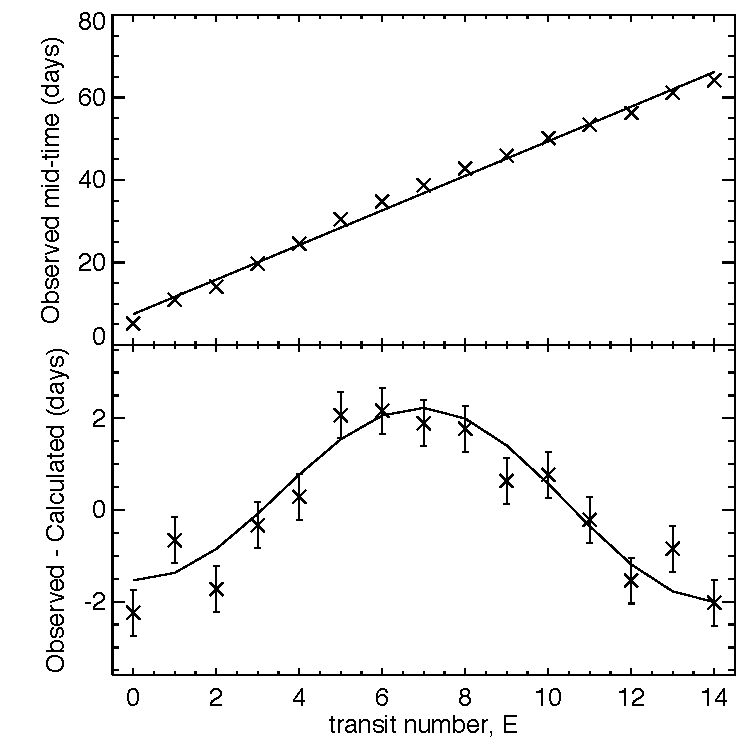
\includegraphics[width=0.9\textwidth]{omc.pdf}}
%
\caption{An example of timing data.  \emph{Top panel}: the measured midtimes of exoplanet transits, to which a line is fit by least-squares.  \emph{Bottom panel}: the residuals of that fit, which is the conventional observed minus calculated ($O-C$) diagram; the original sinusoidal function, to which Gaussian noise was added, is also plotted as a line. }
\label{omc}       % Give a unique label
\end{figure}

The other dynamical effect addressed by this review is TDVs.  Like TTVs, the cause can be changes in $a$, $e$, or $\omega$.  The most dramatic effect, however, is due to orbital plane reorientation.  The angle the orbital plane's normal vector makes to the observer's line of sight --- the inclination --- determines the length of the transit chord.  Changes in the inclination will change the length of that chord, which in turn changes the amount of time the planet remains in transit: duration variations. 

The literature on exoplanets has a history of rediscovering effects that had been well studied in the field of binary and multiple stars.  In the current focus, it has long been known to eclipsing-binary observers that long-term depth changes can result from the torque of a third star orbiting the pair \citep{1971Mayer}.  This effect owes to the secular and tidal dynamics which dominate triple star systems \citep{2003A&A...398.1091B}, dictated by their hierarchical configuration which allows them to remain stable. TDV due to perturbing planets is simply its exoplanetary analogue \citep{2002ApJ...564.1019M}.

The first recognition of the importance of transit timing and duration variations was at the DPS and AAS meetings two decades ago by \citet{1996DPS....28.1208D,1996BAAS...28.1112D}, followed a few years later by \citet{2002ApJ...564.1019M} and \citet{Schneider2003,Schneider2004}.  More detailed studies that included the important effect of mean-motion resonance were independently investigated by \citet{2005Sci...307.1288H} and \citet{2005MNRAS.359..567A}.  The former paper showed that Solar-system like perturbations might be used to find Earth-like planets, should transit times be measured with sufficient accuracy.  The latter paper coined the term `transit-timing variations,' with acronym TTV, and defined TTVs as the observable accumulation of transit period changes (i.e.\ $O-C$).

Initial studies of TTVs of hot Jupiters were able to place limits on the presence of Earth-mass planets near mean-motion resonance \citep{2005MNRAS.364L..96S}.  Some further studies claimed detection of perturbing planets causing TTVs or TDVs, but each of these were quickly disputed or refuted by additional measurements.  The first convincing detection awaited the launch of the \emph{Kepler} spacecraft, and the discovery of Kepler-9 which showed large-amplitude TTVs of two Saturn-sized planets with strong significance \citep{2010Sci...330...51H}; this discovery was remarkably similar to predictions that had been made based upon the GJ 876 system \citep{2005MNRAS.359..567A}.  The Kepler-9 paper kicked off a series of discoveries of TTVs with the \emph{Kepler} spacecraft, with now more than 100 systems displaying TTVs, and a handful showing TDVs \citep{2016ApJS..225....9H}.

\section{Preliminaries}

Since the gravitational interactions between planets occur on the orbital timescale, the
amplitude of TTVs is proportional to the orbital period of each planet,
times a function of other dimensionless quantities.  Thanks to Newton's second law
and Newton's law of gravity, the acceleration of a body does not depend on its own mass.
Thus, the TTVs of each planet scale with the masses of the {\it other} bodies
in the system.
In a two-planet system, then, to lowest order in mass ratio, the $O-C$ formulae are: 
\begin{eqnarray}
\delta t_1 &=& P_1 \frac{m_2}{m_0} f_{12}(\alpha_{12},\mathbf{\theta}_{12}),\cr
\delta t_2 &=& P_2 \frac{m_1}{m_0} f_{21}(\alpha_{12},\mathbf{\theta}_{21}),
\end{eqnarray}
where the masses of the star and planets are $m_0, m_1,$ and $m_2$, and $f_{ij}$ describes the perturbations of planet $j$ on planet $i$,
which is a function of the semi-major axis ratio, $\alpha_{ij} = {\rm min}(a_i/a_j,a_j/a_i)$, and the angular orbital 
elements of the planets, $\mathbf{\theta}_{ij} = (\lambda_i,e_i,\omega_i,I_i,\Omega_i,\lambda_j,e_j,\omega_j,I_j,\Omega_j)$.  The evaluation of these functions can be found in a series of papers on perturbation theory: \cite{2008ApJ...688..636N, 2009ApJ...701.1116N,2010ApJ...709L..44N,2016ApJ...818..177A,2016ApJ...821...96D}.

%  - Linear TTV (independently adds from different planets, off resonance)  - 
With the addition of multiple perturbing planets, if the mass-ratios of the planets to the star are
sufficiently small and if none of the planets exist in a resonant configuration, then the TTVs may be approximately expressed as linear combinations of the perturbations due to each companion.
For $N$ planets, the TTVs become
\begin{equation}
\delta t_i = P_i \sum_{j \ne i}  \frac{m_j}{m_0} f_{ij}(\alpha_{ij},\mathbf{\theta}_{ij}),
\end{equation}
for $i=1,...,N$.

The largest TTVs are caused by orbital period changes associated with librations of the system about a mean-motion resonance, in which the ratio of two planets' orbital periods is close to the ratio of small integers.  We may appeal to energy trades to compute the amplitude of the TTV in each planet (see \citealt{2005MNRAS.359..567A,2010Sci...330...51H}).  Because of Kepler's relation $a \propto P^{3/2}$, a period lengthening of $\delta P_1 \ll P_1$ is associated with a semi-major axis change of $\delta a_1 = (3/2) a_1 \delta P_1 / P_1$.  Differentiating the orbital energy equation $E_1=-G M m_1 /(2a_1)$ shows that such a change results in an energy change of $\delta E_1=(GMm_1 a_1^{-2}/2) \delta a_1$.  To conserve total energy, the other planet will have an energy change of $\delta E_2=-(GMm_1 a_1^{-2}/2) \delta a_1$, which can also be expressed as $+(GMm_2 a_2^{-2}/2)\delta a_2$.  Using the relation $\delta a_2 = (3/2) a_2 \delta P_2 / P_2$, and the Keplerian relation $a_2/a_1=(P_2/P_1)^{2/3}$, we obtain: 
\begin{equation}
\delta P_2 = -\delta P_1 (m_1/m_2) (P_2/P_1)^{5/3}. \label{eqn:deltaP}
\end{equation}
When considering the $O-C$ shapes that each planet makes over a fixed time interval (e.g. from a survey that measures transits for both planets), we will have a factor of $P_2/P_1$ more orbital periods for the inner planet than the outer planet.  Thus the accumulated time shift of the signal, $\delta t$, builds up more for the inner planet, by one factor of the period ratio. In consideration of equation~\ref{eqn:deltaP}, we are left with: 
\begin{equation}
\delta t_2 = -\delta t_1 (m_1/m_2) (P_2/P_1)^{2/3}. \label{eqn:deltat}
\end{equation}
This scaling agrees with analytic work performed in the resonant \citep{2016ApJ...823...72N} and near-resonant \citep{2012ApJ...761..122L,2016ApJ...828...44H} regimes. Hence the TTV curves of the two planets are anti-correlated, and in the case that the masses are equal, the amplitude of the outer planet's TTV is larger because its orbital size needs to change more for its Keplerian orbital energy to equal the change in the inner planet's Keplerian orbital energy. 

In general, transit timing variations afford a means of measuring the density of exoplanets.
The two observables associated with a light curve are the time stamp of each photometric
measurement and the number of photons measured.  The number of photons is a dimensionless
number, and thus may only constrain dimensionless quantities, such as radius ratio, impact 
parameter, or the ratio of the stellar size to the semi-major axis.  The quantities that 
have units of time --- the period, transit duration, ingress duration ---  can 
constrain the density of the system since the dynamical time relates to stellar density, $\rho$, as
$t_{dyn} \approx (G\rho)^{-1/2}$.  \citet{2003ApJ...585.1038S} showed that a single transiting planet
on a well-measured circular orbit may be used to gauge the density of the star;
in the case of multiple transiting planets, the circular assumption may be relaxed
\citep{2014MNRAS.440.2164K}.

The transit depth, then, gives the radius-ratio of the planet to the star, while if two planets
transit and show TTVs, their TTVs give an estimate of the mass ratio of the perturbing planet
to the star.  Thus, two transiting, interacting planets yield an estimate of the density ratio of
the planets to the star, and consequently we can obtain the density of the planets.
Note that this is true even if the absolute mass and radius of the star are poorly
constrained.  A caveat to this technique is that there is an eccentricity dependence that 
is present in the stellar density estimate.  However, multi-transiting planet systems typically require low eccentricities to be stable,
and in some cases the eccentricities can be constrained sufficiently from TTV analysis, from
analyzing multiple planets \citep{2014MNRAS.440.2164K}, or
from statistical analysis of an ensemble of planets \citep{Hadden2017}.  So this caveat ends up not impacting the stellar density 
estimate significantly (the mass-eccentricity degeneracy, however, reduces precision on planet-star mass ratios, and hence inflates the planet density uncertainty). 
Another way to obtain an estimate of stellar density is from asteroseismology:
in fact, the time-dependence of asteroseismic measurements is what enables density
to be constrained in that case as well \citep{1986ApJ...306L..37U}.

If a pair of transiting exoplanets can be detected with {\it both} TTVs and RVs, then the
absolute dimensions of the system may be obtained \citep{2005MNRAS.359..567A,
2013ApJ...762..112M} as RVs have dimensions of velocity, which 
when combined with time measurements from TTVs gives dimensions of distance.
In practice this technique has yet to yield useful constraints upon the properties
of planetary systems \citep{2015MNRAS.453.2644A}, but it may prove fruitful
in the future much as double-lined spectroscopic binaries have used to measuring 
the properties of binary stars, as hinted at by \cite{2016A&A...595L...5A}.  Circumbinary planets 
(CBP) are an extreme example of this technique: the timing offsets of the transits, combined with the eclipses
and radial-velocity of the binary give very precise constraints on the absolute parameters
of the Kepler-16 system \citep{2011Sci...333.1602D}.

\section{Theory and Paradigmatic Examples} 

Here we discuss the physical models for different types of TTV interactions, and point the reader to real systems that exhibit each kind of interaction. 

Close to resonances, a combination of changes in semi-major axis and eccentricity lead to TTV cycles whose period depends on the separation from the resonance \citep{Steffen2006,2012ApJ...761..122L}; the latter refer to this as the `super-period.'  The main TTV variation comes from only one resonance, the one the system is closest to, which allows its critical angles to move slowly and thus its effect to build up.  If the period ratio $P_2/P_1$ is within a few percent of the ratio $j/k$, with $j$ and $k$ being integers, then the expected TTV period is 
\begin{equation}
P_{\rm TTV} = 1/|j/P_2-k/P_1|. \label{eqn:pttv}
\end{equation}
The order of the resonance is $|j-k|$, and the strength of the resonance depends on the planetary eccentricities to a power of the order minus 1.  Therefore, first order resonances affect planets with no initial eccentricity, but higher order resonances have a large effect only in the presence of some eccentricity. 

Seeing two planets transit the star helps immensely to characterize a near-resonant system, because then the relative transit phase of the two planets can be compared with the phase of the TTV signals \citep{2012ApJ...761..122L}.  If the eccentricities are maximally damped out, then the resonant terms of the interaction continue forcing a small eccentricity that quickly precesses, causing the TTV.  In that case, the phase of the signal is predictable, and the two planets' eccentricities are anti-aligned, so the TTV signals consist of anti-correlated sinusoids.  Also useful in that case is that the amplitudes lead directly to the planetary masses.  If so-called ``free eccentricity'' remains, however, the phases would usually differ from that prediction, the TTV in the two planets may not be in perfect anti-phase, and only an approximate mass scale rather than a measurement is available, which is referred to as the mass-eccentricity degeneracy.  The first real system that showed this pattern convincingly was Kepler-18 \citep{2011ApJS..197....7C}. %[figure of that rather than the theory one given currently in figure 2?]. 
The degeneracy between mass and eccentricity results from sampling at the period of the transiting planet, which causes short period variations to be aliased with $P_{TTV}$ \citep{2012ApJ...761..122L,2015ApJ...802..116D}.  

The measurement of TTVs and TDVs has been used for confirmation, detection, and characterization of
transiting exoplanets and their companions.  The \emph{Kepler} spacecraft discovered thousands of transiting
exoplanet candidates;  the classification as `candidate' was cautiously used to allow for other
possible explanations, such as a blend of a foreground star and a background eclipsing binary causing
an apparent transit-like signal.  The presence of multiple transiting planets around the same star
gave a means of confirming two planets that display {\em anti-correlated} TTVs: due to energy conservation (equation~\ref{eqn:deltat}), the anti-correlation indicates dynamical interactions between the
two planets, while such a configuration would not be stable for a triple star system.  Many papers
used this technique to confirm that \emph{Kepler} planet candidates were bonafide exoplanets using different techniques to identify the anticorrelation in data \citep{2012ApJ...750..113F,2012ApJ...756..185F,2012ApJ...750..114F,2012MNRAS.421.2342S,2013ApJS..208...22X}.

The characterization of exoplanets with TTVs also began in earnest with the \emph{Kepler} spacecraft.
In addition to Kepler-9, the Kepler-18 system was characterized by a combination of TTVs and
RVs, giving density estimates for the three transiting planets \citep{2011ApJS..197....7C} and assuring that the new method for mass characterization gave the same answers as the trusted, older method.

When only one planet transits in a near-resonant system, the measured TTVs may simply record a sinusoidal signal, which could result from the other planet being close to many different resonances with the transiting planet \citep{2010ApJ...718..543M}.  In Kepler-19, \cite{2011ApJ...743..200B} were able to tell that a planetary companion was the only sensible cause of the TTV, but they were not able to break this finite set of degeneracies. 

This degeneracy has made it extremely difficult to characterize non-transiting planets via TTV, and hence in many cases an additional planet is suspected due to TTV, but detailed work has not been pursued to determine its nature.  The first case of a non-transiting planet being discovered \emph{and} completely characterized was Kepler-46 (a.k.a. KOI-872; \citealt{2012Sci...336.1133N}).  The authors found that the TTVs of the transiting planet were far from a sinusoidal shape; in fact, they could be Fourier-decomposed into at least four significant sinusoids.  Each of these sinusoids can be identified as the interaction with the non-transiting planet via a different resonance.  Even with all this extra information, TTVs could only narrow down the possible perturbing planets to a degenerate set of two.  The clever solution \citep{2012Sci...336.1133N} was to note that one of those solutions, to get the relative amplitudes of the component sinusoids correct,  requires the perturbing planet to be somewhat inclined with respect to the transiting planet.  As a consequence, a torque on that planet would drive TDV.  No such TDV were observed, so the unique solution was found. 

Planets that are truly in resonance with each other have the largest TTV signals.  On a medium-baseline timescale like that of \emph{Kepler}, they can perturb each other's orbital periods.  The resonant interaction traps the planets at a specific period ratio, causing the periods to oscillate near that ratio.  The period of the full cycle of that oscillation depends on the ratio of the planet masses to the host star's mass, to the $-\nicefrac{2}{3}$ power \citep{2005MNRAS.359..567A,2016ApJ...823...72N}.  For instance, the touchstone system GJ876 has a 550 day libration cycle, about 10 times the outer planet's period, due to its relatively massive planets and low-mass star.  A system which was characterized by resonant interaction is KOI-142 \citep{2013ApJ...777....3N}, in which a non-transiting planet was discovered.   A system with two transiting planets in resonance with large TTVs is Kepler-30 \citep{2012ApJ...750..114F}.  A system with smaller libration amplitudes, but a surprising \emph{four} planets in resonance (forming a chain of resonances) is Kepler-223 \citep{2016Natur.533..509M}.

Several other TTV mechanisms have been detected which do not rely on resonances, but are relevant for more hierarchical situations ($P_2/P_1 \gtrsim 4$). 

If the outer planet transits, and the inner orbiting body is very massive, the dominant effect can be the shifting of the primary star with respect to the barycenter.   Then, as the outer planet orbits the barycenter, it arrives at the moving target either early or late.  This effect was numbered (i) by \cite{2005MNRAS.359..567A}, and it is seen clearly in circumbinary planet systems.  For instance, the secondary star of Kepler-16 \citep{2011Sci...333.1602D} moves the primary by many times its own radius, resulting in an $\sim 8$~day TTV on top of a 225 day orbit. 

A final mechanism of dynamical TTV is relevant for the inner orbit when a massive body orbits at large distance.  The tide that body exerts on the inner orbit causes its orbital period to differ slightly from what it would be in the absence of that outer body.  If the outer body is in the plane of the inner orbit, its tide slows down the inner orbit, lengthening its period.  If the outer body is far out of the plane of the inner orbit, its tide speeds up the inner orbit, shortening its period.  The tide also depends on the third power of the distance to that external body.  Hence, when the external body moves on an eccentric and/or inclined orbit, it induces a period variation in the inner orbit, which has the period of the outer orbit.  Also imporant for the timing is how the outer perturber instantaneously torques the inner orbit's eccentricity.  These effects were put together and analyzed by \cite{2003A&A...398.1091B} in the context of triple star systems, and the in-plane physics was explained as mechanism (ii) of \cite{2005MNRAS.359..567A}.  An example of these effects was provided by Kepler-419 \citep{2014ApJ...791...89D}, in which an eccentric massive planet accompanies an inner planet with a period ratio of 9.7.

\subsection{Chopping}

When two planets are nearly resonant, the degeneracy between the mass ratios of the planets to the star
and the eccentricity vector may be broken by examining additional TTV components present in the data \citep{2015ApJ...802..116D}.
Non-resonant perturbations occur on the time from one conjuction of the planets to the next, which is
when their separation is smallest and gravitational attraction is strongest.  Conjunctions
occur on a period of $P_{\rm syn}= (1/P_1-1/P_2)^{-1}$, also referred to as the synodic period.
TTVs at the synodic period, and its harmonics, have smaller amplitude due to 
the fact that they do not add coherently, and thus require higher signal-to-noise to detect.
These synodic variations are referred to as ``chopping" as they commonly
show TTVs that alternate early and late, on top of the larger amplitude TTVs with period $P_{TTV}$.
Despite the smaller amplitude, the chopping components can be detected in many cases, and can break
the mass-eccentricity degeneracy, leading to a unique measurement of the masses of the exoplanets 
\citep{2014ApJ...790...58N,2014ApJ...795..167S,2015ApJ...802..116D}.

As an example, consider a pair of planets with period ratio of $P_2/P_1 = 1.52$.  This period ratio
is close to 3:2, and thus is affected by this resonant term, giving a TTV period of $38 P_1$ by equation~\ref{eqn:pttv}.
Figure \ref{ttv_chopping} compares two planets with this period ratio with zero eccentricity
and mass-ratios of $10^{-6}$ to a pair of planets with eccentricites of $e_1=e_2=0.04$
and mass-ratios near $10^{-7}$.  Both pairs of planets give nearly identical amplitudes
for the large resonant term due to the mass-eccentricity degeneracy discussed above, while the larger mass ratio planets show a 
much stronger chopping variation.  In this case there is a clear difference between the TTVs of the two simulated
systems:  the inner planet shows a drift over three orbital periods, and a sudden jump
every third orbital period, while the outer one shows a similar pattern over two orbital
periods.  
In this example the phase of the orbital parameters are set such that the TTV amplitudes match;  change
in the phase can also be indicative of a non-zero eccentricity contributing to the TTVs,
and with an ensemble of planets which are believed to have a similar eccentricity
distribution, the mass-eccentricity degeneracy may be broken statistically \citep{2012ApJ...761..122L,
2014ApJ...787...80H}.

% For figures use
\begin{figure}
\centerline{
\includegraphics[width=0.9\textwidth]{ttv_chopping.pdf}}
%
\caption{Transit-timing variations of two low-eccentricity planets with larger
mass ratios, $m_1 = m_2 = 10^{-6} m_*$ (green) compared with two higher eccentricity planets ($e_1=e_2=0.04$)
with smaller mass ratios $m_1 = m_2 = 10^{-7} m_*$.  The zig-zag chopping component
is apparent in the high-mass/low-eccentricity case, while less apparent in the low-mass/
high-eccentricity case.}
\label{ttv_chopping}       % Give a unique label
\end{figure}



\subsection{Transit Duration Variations}

TDVs have given useful results for characterization of individual systems, though fewer in number than TTVs.  Two mechanisms for TDV have been observed in planetary system orbiting a single primary star.  The first is torque due to the rotational oblateness of the star.  It is a convincing model for the duration changes in Kepler-13 b \citep[KOI 13.01][]{Szab2012} and a controversial explanation for transit shape anomalies in PTFO 8-8695 \citep{2013ApJ...774...53B}.  The second planetary cause of TDVs is dramatic eccentricity variations due to a resonant interaction.  The length of the chord across the star, as well as the speed at which the planet moves along that chord, are changed during the planetary interaction.  This effect has been observed in KOI-142 \citep{2013ApJ...777....3N}.  Finally, it has not been measured yet for planets orbiting single stars, but slow secular precession of the eccentricity is expected by general relativity \citep{2008MNRAS.389..191P}, by stellar oblateness \citep{2007MNRAS.377.1511H}, and by tidal distortion \citep{2009ApJ...698.1778R}.  It is likely that very long time-baseline measurements, or comparing the measurements of two time-separated space missions like Kepler and Plato, will be able to detect this effect.

More dramatic dramatic TDVs can occur in circumbinary planet systems due to the moving-target effect described above for TTVs.  If the transit occurs while the star is moving in the same direction as the planet, the transit duration is longer; if in opposite directions, the transit duration is shorter.  Matching the prediction from the phase of the binary completely secures the interpretation of the signal that an object is in a circumbinary orbit, as discussed extensively by \cite{2013ApJ...770...52K} for the cases of Kepler-47 and Kepler-64 (a.k.a. PH-1, KIC 4862625b).

Just as in several known cases of stellar triples, the precession of CBPs has caused transits to turn on and off \citep{2017MNRAS.465.3235M}.  The first case of that phenomenon was Kepler-35 \citep{2012Natur.481..475W}, and the most spectacular so far observed was Kepler-413 \citep{2014ApJ...784...14K}, in which a $4^\circ$ mutual inclination caused transits to stop and then start again nearly half a precession cycle later.  Planetary torques also cause TDV, albeit on a longer timescale through changing the inclination.  This was observed in Kepler-117 \citep{2015MNRAS.453.2644A} as well as Kepler-108 \citep{1538-3881-153-1-45}, the latter indicating mutual inclination of $\sim 15^\circ$ in a rather hierarchical pair of planets. 

Two other mechanisms for TDV have been observed in planetary systems orbiting a single primary star.

The first is torque due to the rotational oblateness of the star.  It is a convincing model for the duration changes in Kepler-13 b \citep[KOI 13.01][]{Szab2012} and a controversial explanation for transit shape anomalies in PTFO 8-8695 \citep{2013ApJ...774...53B}. 

The last planetary cause of TDVs is dramatic eccentricity variations due to a resonant interaction.  The length of the chord across the star, as well as the speed at which the planet moves along that chord, are changed during the planetary interaction.  This effect has been observed in KOI-142 \citep{2013ApJ...777....3N}.

Finally, it has not been measured yet, but slow secular precession of the eccentricity is expected by general relativity \citep{2008MNRAS.389..191P}, by stellar oblateness \citep{2007MNRAS.377.1511H}, and by tidal distortion \citep{2009ApJ...698.1778R}.  It is likely that very long time-baseline measurements, or comparing the measurements of two time-separated space missions like \emph{Kepler} and \emph{Plato}, will be able to detect this effect.

\section{Observational considerations: timing precision} % EA

The steepest portions of a transit are the ingress and egress when the planet crosses onto and
off of the disk of the star, causing a dip of depth $\delta = (R_p/R_*)^2$ if limb-darkening is ignored.   
Suppose for the moment that the only source of noise is Poisson noise due to the count rate of 
the star, $\dot N$.  The photometric uncertainty over the duration of ingress, $\tau$ (eqn.\ \ref{ingress}), 
scales as $(\dot N \tau)^{1/2}$.  If the time of 
ingress fit from a model is offset by $\sigma_\tau$, then the difference in counts observed
versus the model is $\sigma_\tau \delta \dot N$ (the pink region in Fig.\ \ref{fig:ingress}).  Equating 
this count deficit to the photometric uncertainty gives $\sigma_\tau = \tau^{1/2} \dot N^{-1/2} \delta^{-1}$, which
is the 68.3\% confidence timing precision assuming that the exposure time is much shorter than the
ingress duration and that $\sigma_\tau \ll \tau$.  The same formula applies to egress. A longer transit 
ingress duration leads to a shallower slope in ingress, which makes it more difficult to measure an 
offset in time of the model.  Higher count rates and deeper transits improve the precision, as 
expected.  Note that we've assumed that the duration of the transit is sufficiently long that the 
error on $\delta$ is small.

Suppose the transit duration is $T$.  Then, the uncertainty on the duration is given by
the sum of the uncertainties on the ingress and egress, added in quadrature:
$\sigma_T = \sqrt{2} \sigma_\tau$.  The timing precision, $\sigma_t$, is set by the mean of the ingress
and egress, giving $\sigma_t = \frac{1}{\sqrt{2}} \sigma_\tau$.

A more complete derivation of these expressions is given by \citet{2008ApJ...689..499C}, while an 
expression which includes the effects of a finite integration time is given by \citet{2014ApJ...794...92P}.
The assumptions of no limb-darkening and Poisson noise are generally broken by stars;  in addition,
stellar variability contributes to timing uncertainty, for which there is yet to be a general
expression.  These effects generally increase the uncertainty on the measurement of transit times
and durations, and so the best practice would be to estimate the timing uncertainties from the
data, accounting for effects of correlated stellar variability by including the full covariance
matrix of the timing uncertainty \citep{2009ApJ...704...51C,2012MNRAS.419.2683G,ForemanMackey2017}.  Crossing of
the path of the planet across star spots may also cause some uncertainty on the timing precision 
\citep{2013A&A...556A..19O,2013MNRAS.430.3032B};
this can be diagnosed by a larger scatter within transit than outside transit or other signs of
significant stellar activity, and can be handled best by including the spots in the transit model 
\citep{2016A&A...585A..72I}.

Note that the barycentric light-travel time offset must be corrected for carefully for high-precision
TTV \citep{2010PASP..122..935E}.

% For figures use
\begin{figure}
% Use the relevant command for your figure-insertion program
% to insert the figure file.
% For example, with the graphicx style use
\centerline{
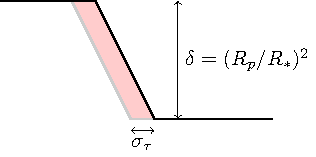
\includegraphics[width=0.5\textwidth]{ingress.pdf}}
%
\caption{Diagram of the transit ingress of a planet, flux versus time.  The precision of the timing of ingress, $\sigma_\tau$, is set by
when the area of the ingress (pink) equals the timing precision over the duration of ingress. The same applies to egress, albeit
with the time flipped in this plot.}
\label{fig:ingress}       % Give a unique label
\end{figure}

\section{Science Results}

The best characterized pair of small planets to date using TTV reside in the Kepler-36 system \citep{2012Sci...337..556C}.  As this planet pair is in close proximity, the conjunctions cause a significant kick to each planet resulting a TTV amplitude that is $\approx 1$\% of the orbital periods of the planets.  Figure \ref{fig:kep36} shows a `river-plot' for all seventeen quarters of long-cadence \emph{Kepler} data for this pair of planets.  After each 7(6) orbits of the inner(outer) planet (or so), there is a conjunction which causes a change in the eccentricity vector and period of each planet.  The change in the eccentricity vector causes a sudden change in the subsequent transit time, while the change in period causes a change in slope;  these are apparent for Kepler-36c in Figure \ref{fig:kep36}.  The large TTVs enable a precise measurement of the planet-star mass ratios for both planets (using the TTVs of the companion planet), while the star shows asteroseismic variability which gives a precise estimate of the stellar mass.   The result are masses with uncertainties of $<8$\%, which is the most precise to date for planets of approximately this mass or lower, $4.5\pm 0.3$ and $8.1 \pm0.6  M_\oplus$.  The inner planet shows a density which is consistent with scaling up in mass a planet of the composition of Earth, while the outer planet requires a significant H/He envelope to explain its size which is comparable to Neptune \citep{2012Sci...337..556C}.

\begin{figure}
\centerline{
\includegraphics[width=0.9\textwidth]{kepler36.pdf}}
\caption{River plot of Kepler-36b (left) and Kepler-36c (right). Each row of each panel shows the intensity
of the star scaled with color and centered on the mean ephemeris of each planet.}
\label{fig:kep36}
\end{figure}

A wide-spread phenomenon was detected by TTV characterization of masses: the existence of puffy sub-Neptune planets.  In the first such case, Kepler-11 e \citep{2011Natur.470...53L}, a planet with a mass half of Neptune's has a size slightly bigger than Neptune.  Even more extreme cases of this class have been found, the most extreme which we consider secure is a $2.1^{+1.5}_{-0.8} M_\oplus$ planet with a radius of $7 R_\oplus$ in Kepler-51 \citep{2014ApJ...783...53M}.  These massive envelopes mean these low-mass planets formed while gas was still present in the protoplanetary disk, and that they were able to capture that gas, a surprising result \citep[e.g.][]{2016ApJ...817...90L,2016ApJ...825...29G}. 

Catalogs of transit times have been produced for the multi-planet \emph{Kepler} systems \citep{2013ApJS..208...16M,Rowe2015,2016ApJS..225....9H}. Several analyses of an ensemble of TTV pairs of planets have recently been carried out \citep{2014ApJ...787...80H,2013ApJS..208...22X,2014ApJS..210...25X,2016ApJ...820...39J}, with the largest by Hadden \& Lithwick (2016), yielding constraints on the RMS eccentricity of the population of planets.  A slightly smaller sample, selecting only planets with mass precisions of better than $3-\sigma$, yields Figure \ref{fig:density_period}.  There appears to be a trend of mean density decreasing with orbital period (one exception is K2-3d, although the authors warn its RV mass estimate may be affected by stellar variability).  At periods near $\approx 10$ days, the RV and TTV densities agree rather well.  At shorter period, most of the RV detections are single-planets, which in general appear to have lower density relative to their multi-planet counterparts \citep{Steffen2016,2017ApJ...839L...8M}.  When radius is plotted versus mass, and color-coded as a function of flux, Fig.\ \ref{fig:density_period}, there is a general trend of radius increasing with mass, albeit with a large scatter in mass, while a handful of `puffy' planets (with masses measured with TTV) show shockingly large radii given their small masses.  These mass measurements are surprising, but difficult to dispute as larger masses would have led to a larger, and hence easier-to-measure, TTV signal.

\begin{figure}
\centerline{
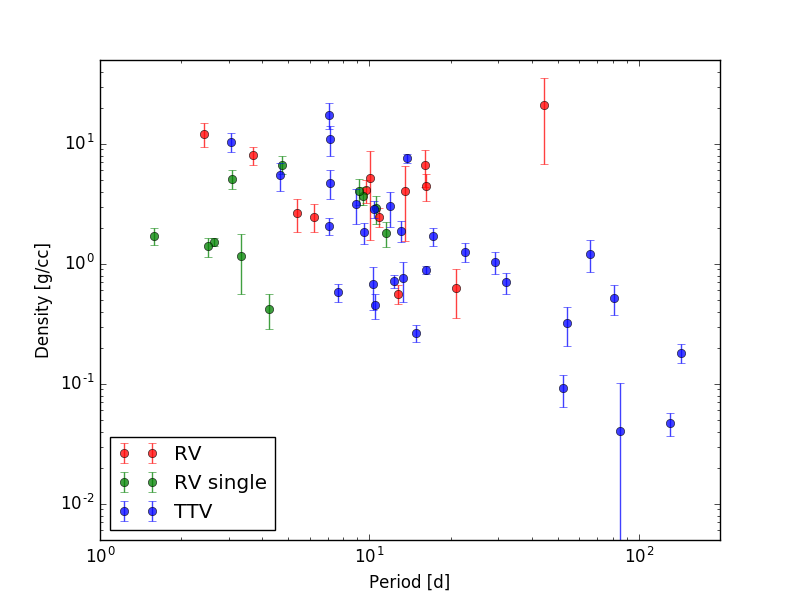
\includegraphics[width=0.95\textwidth]{density_vs_period_errors.png}}
\centerline{
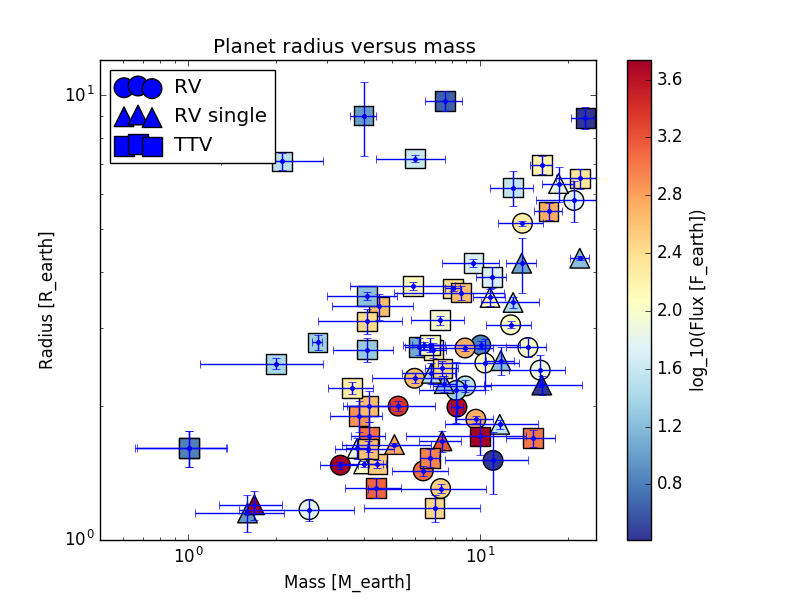
\includegraphics[width=0.95\textwidth]{mass_radius_flux.png}}
\caption{Density vs.\ period for planets transiting planets with masses $<25 M_\oplus$ (left).  Radius
vs.\ mass, with color indicating incident stellar flux (right).}
\label{fig:density_period}
\end{figure}

With the end of the primary \emph{Kepler} mission, the data volume of transit times has diminished.
Nevertheless, the K2 mission has continued to provide TTV systems such as WASP-47, the first
short-period hot Jupiter with nearby planet companions \citep{2015Becker}.  The surprising discovery
of seven planets orbiting a late-type star, TRAPPIST-1, also displays signifincant TTVs which
will be used to precisely characterize the densities of these small exoplanets \citep{2017Natur.542..456G}.
With the launch of TESS in 2018 \citep{2015JATIS...1a4003R}, transit timing will enhance the analysis 
of the multi-planet systems found, especially near the polar regions with longer term coverage, 
or when followed up with CHEOPS \citep{2014PASP..126.1134B}. 
The PLATO mission next decade will cause another spike in TTV science \citep{2014ExA....38..249R},
as will possibly WFIRST \citep{2017PASP..129d4401M}. The James Webb Space Telescope may allow the
extension in time baseline and increase in precision for high-priority transit-timing targets 
\citep{2014PASP..126.1134B}.  All to say, the future of characterizing multi-transiting planet
systems with TTV (and TDVs) looks promising.


\begin{acknowledgement}
EA acknowledges support from NASA Grants NNX13AF20G, NNX13A124G, NNX13AF62G, from National Science Foundation (NSF) grant AST-1615315, and from NASA Astrobiology Institute's Virtual Planetary Laboratory, supported by NASA under cooperative agreement NNH05ZDA001C.  DCF acknowledges support from NASA under Grant No. NNX14AB87G issued through the \emph{Kepler} Participating Scientist Program and from the Alfred P. Sloan Foundation.  We thank Sam Hadden, Jack Lissauer, Kento Masuda, Mahmoudreza Oshagh, and Jason Steffen for feedback, and we thank the Other Worlds Laboratory at UC Santa Cruz for hospitality while revising this paper.
\end{acknowledgement}

%  IF you do NOT use bibtex, put comments before the following 2 lines
\bibliographystyle{spbasicHBexo}  %for bibtex
\bibliography{agol_fabrycky} %for bibtex-example

\end{document}
